\documentclass{article}
\usepackage[utf8]{inputenc}
\usepackage{hongli_latexpack}

\title{Autumn 2022 STAT 31120 Solutions}
\author{Hongli Zhao}
\date{November 2022}
\begin{document}

\maketitle
\begin{abstract}
    STAT 31120 / CAAM 31120 at the University of Chicago is a graduate-level course on Numerical Methods for Stochastic Differential Equations. The course covers fundamental concepts concerning strong and weak convergence of random variables, stochastic Taylor expansions (Taylor-Ito expansion), difference between Ito and Stratonovich integrals, and explicit numerical methods for stochastic integration. I had the fortune to work closely with \href{https://www.stat.uchicago.edu/~zhongjian/}{Prof. Zhongjian Wang} as the course reader for Winter 2021 and Autumn 2022 offerings of the course. The course webpage is updated \href{https://www.stat.uchicago.edu/~zhongjian/courses/stat31120_2022aut/CourseHomepage.html}{here}. Textbook used was Kloeden \& Platen, \emph{Numerical Solution of Stochastic Differential Equations.}
    
    This document details updated solutions to course projects (5 in total) along with a small portion of the final. Code is available on the associated Github page, in Python and Julia. Any comments and suggestions are welcome, please send an email to \texttt{honglizhaobob@uchicago.edu}.

    \emph{Disclaimer}: If you are viewing this document (or Github page) as an active UChicago student, please use this document at your own risk, add appropriate references, and adhere to UChicago's academic integrity policy. Please email me or your course instructor if you are unsure.
\end{abstract}

\section{Project 1}
\subsection{Uniform Random Number Generation} 

\noindent \indent Generate $N = 10^4$ uniformly distributed pseudo random numbers on $(0,1)$. Partition the interval into subintervals $I_j$ of equal length 0.05. Count the number of random numbers in $I_j$ as $N_j$. Plot the relative frequencies:
$$
    p_j = \frac{N_j}{N\cdot I_j}
$$ to create a histogram. Compare this histogram with the density of $U(0,1)$. 

In addition, compute sample average and sample variance and compare them to the exact expectation and variance $1/2$ and $1/12$.

\emph{Solution}: The Julia code for creating histogram and computing moments of $\mathcal{U}[0,1]$ is as follows.
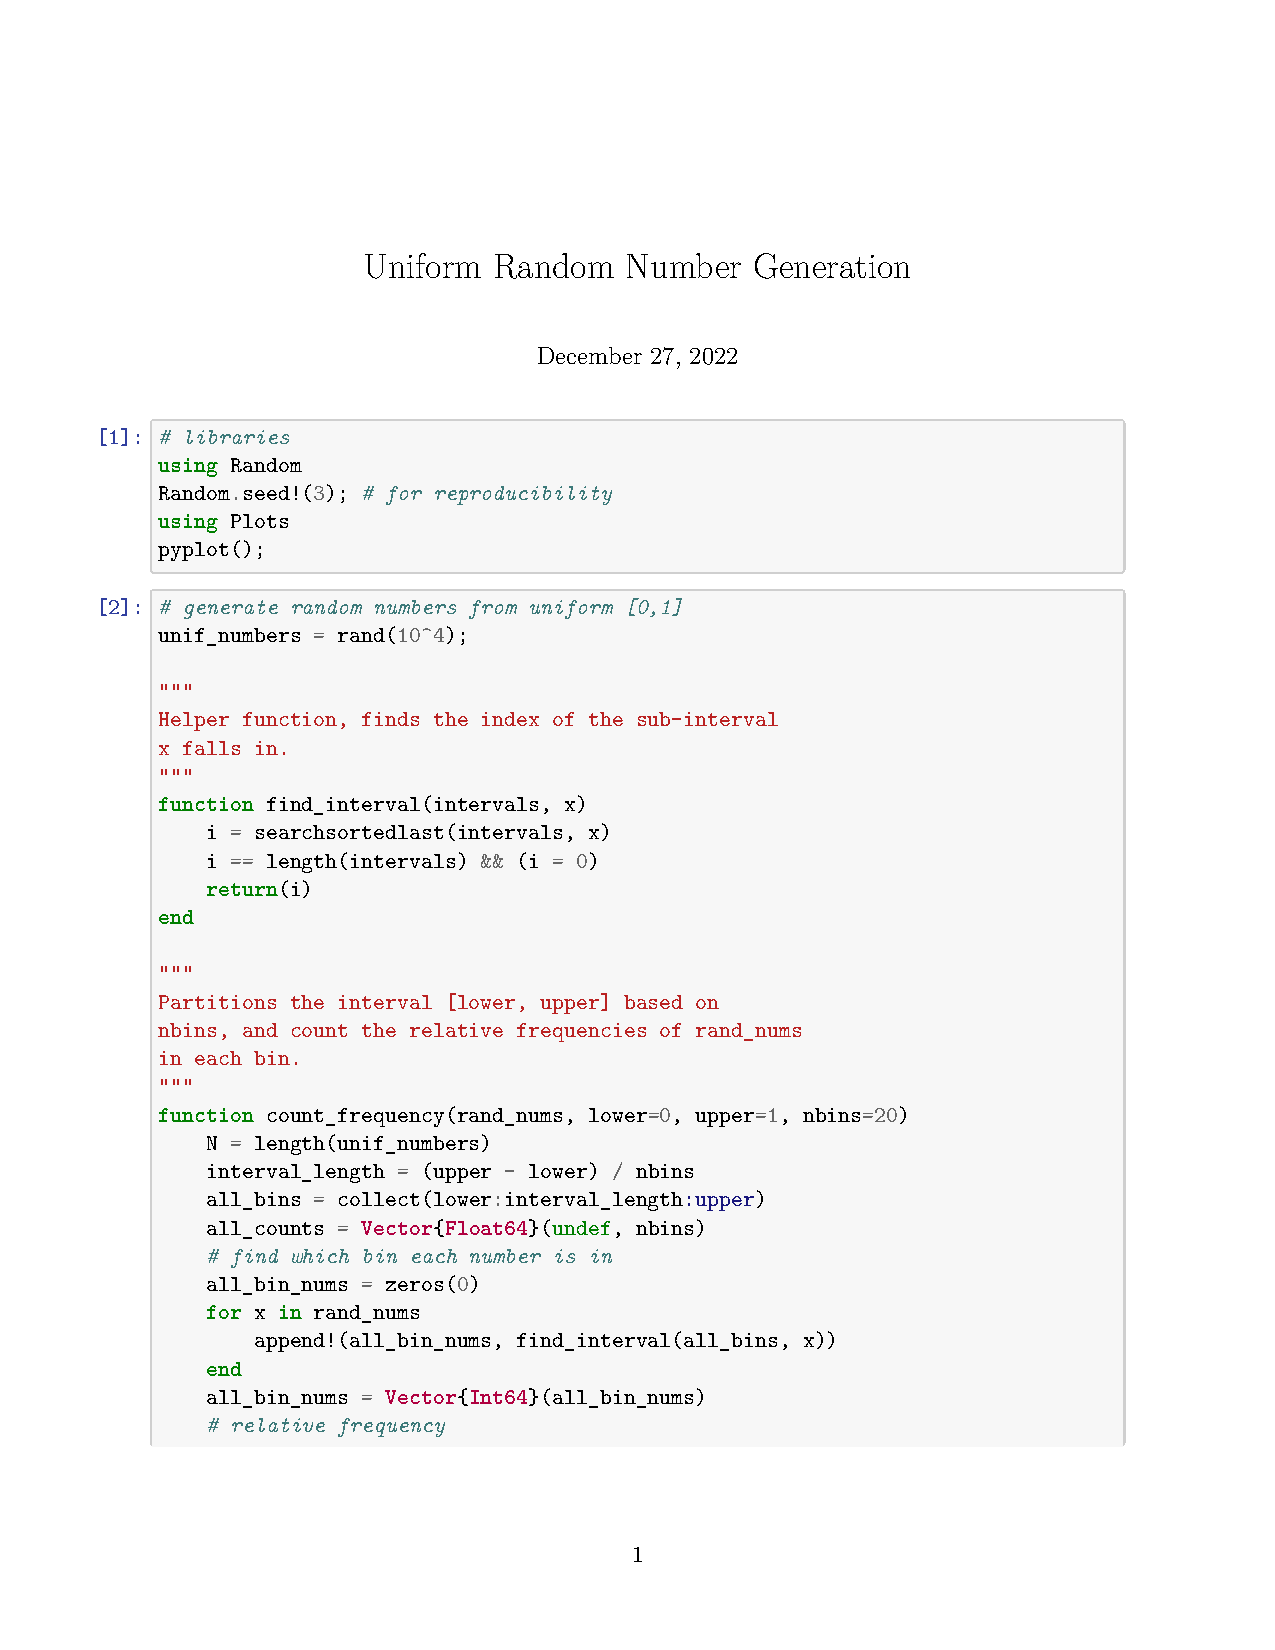
\includepdf[pages=-]{./proj1/Uniform Random Number Generation .pdf}

\subsection{Custom Density Random Number Generation} \indent \indent Repeat the previous question for the following density supported on $[0,2]$.
$$
    p(x) = \frac14x^3
$$

\emph{Solution}: We first verify the theoretical mean and variance for $p$. Let $X\sim p$
$$
    \expect{X} = \int_0^2xp(x)dx = \frac14\int_0^2x^4dx = \frac85
$$ similarly, 
$$
    \expect{X^2} = \frac83, \text{Var}[X] = \expect{X^2} - \expect{X}^2 = \frac{8}{75}
$$

To sample from the distribution $p$, we generate random seeds from $\mathcal{U}[0,1]$ and apply the inverse CDF method. The CDF is given by:
$$
    P(x) = \int_0^xp(z)dz = \frac{1}{16}x^4
$$ then $P^{-1}(z) = 2z^{1/4}$ for $z\sim \mathcal{U}[0,1]$. The code for generating the samples are as follows.
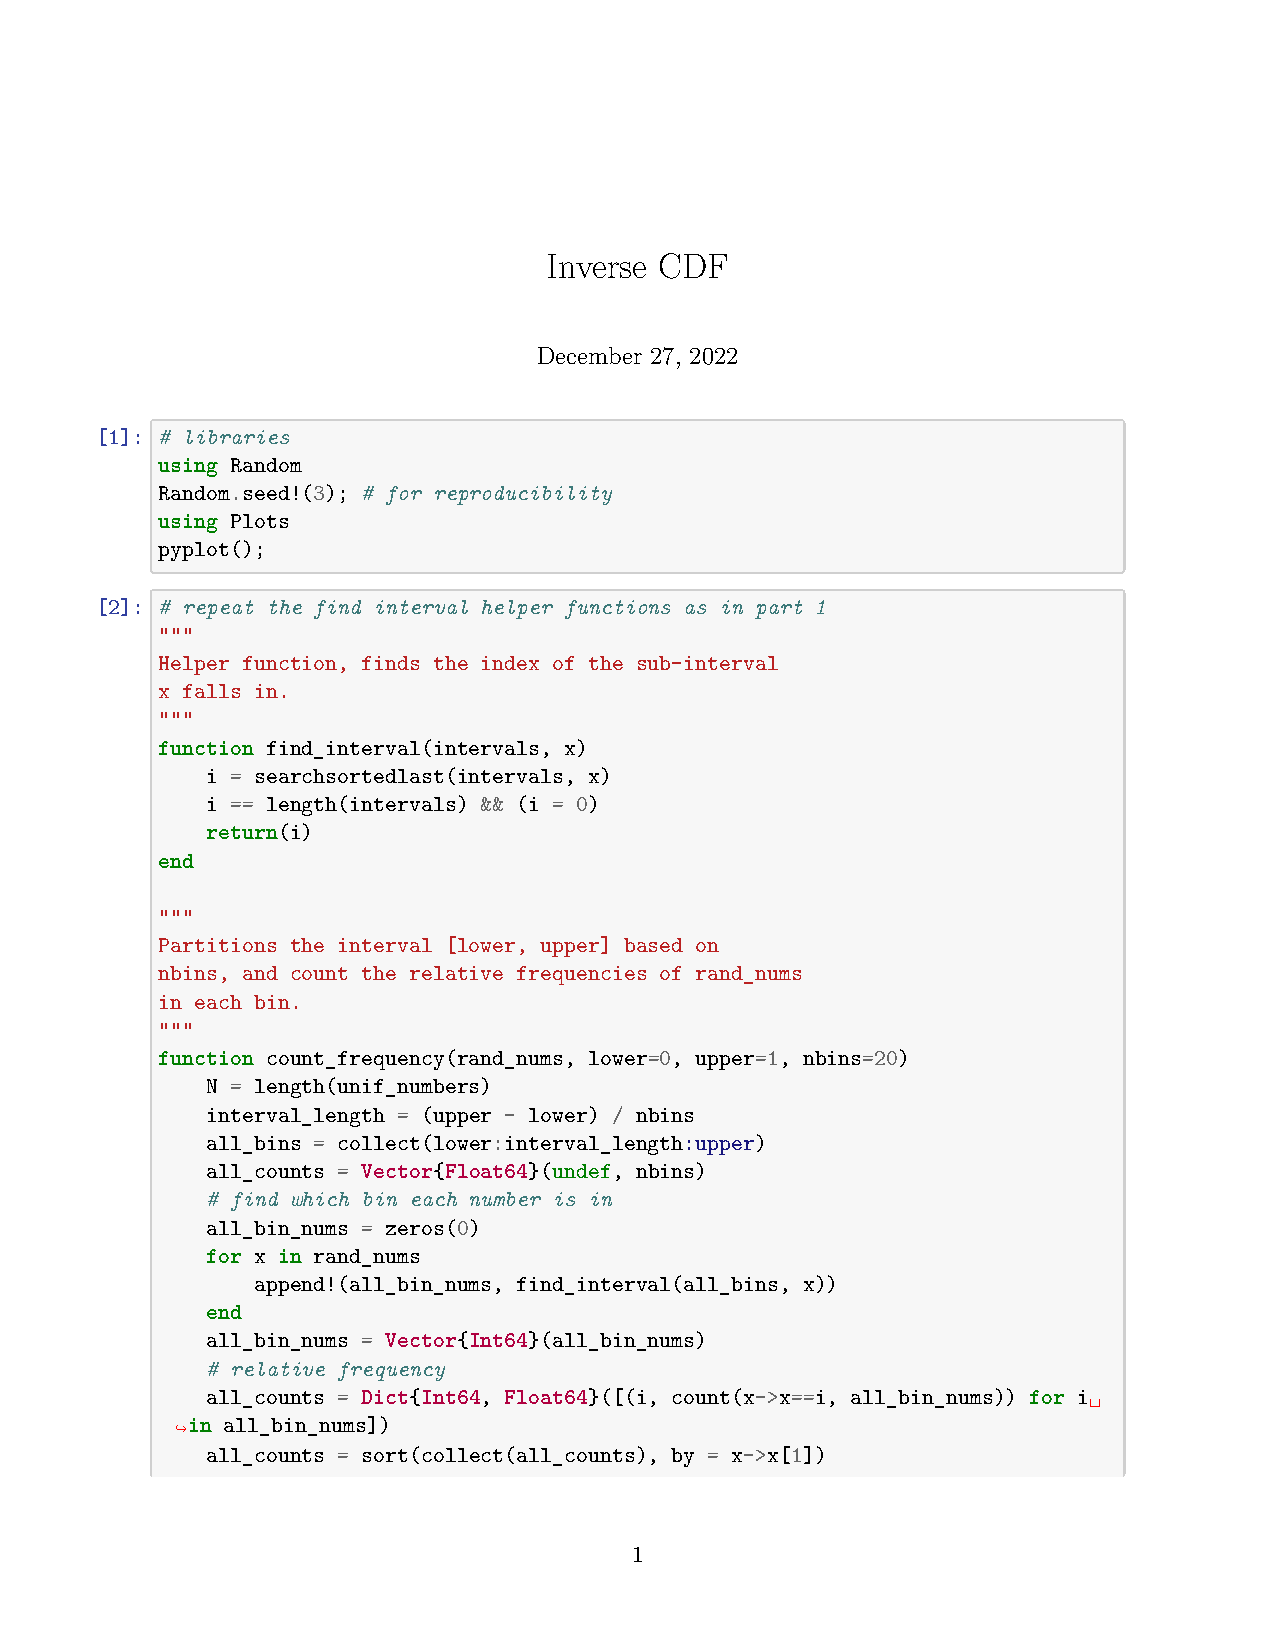
\includepdf[pages=-]{proj1/Inverse CDF.pdf}

\subsection{Box-Muller Distribution} Show that two random numbers $N_1, N_2$, generated by the Box-Muller method, are Gaussian with zero mean and identity variance, when the seeds $U_1,U_2$ are independent $U(0,1)$ distributed. 

\emph{Solution}:

The Box-Muller method uses the following nonlinear mapping:
$$
    N_1 = \sqrt{-2\ln U_1}\cdot \cos(2\pi \cdot U_2)
$$
$$
    N_2 = \sqrt{-2\ln U_1}\cdot \sin(2\pi \cdot U_2)
$$ where $U_1,U_2$ are $\text{Unif}[0,1]$.

Consider polar coordinates defined by:
\begin{eqnarray*}
    r = \sqrt{N_1^2 + N_2^2} = \sqrt{-2\ln U_1\cdot \cos^2(2\pi \cdot U_2) - 2\ln U_2 \cdot \sin(2\pi \cdot U_1)} \\
    = 
    \sqrt{-2\ln U_1}(\cos^2(2\pi U_2) + \sin^2(2\pi U_2)) = \sqrt{-2\ln U_1}\\
    \theta = \tan^{-1}(\frac{N_2}{N_1}) = \tan^{-1}\bigg[
        \frac{\sin(2\pi \cdot U_2)}{\cos(2\pi\cdot U_2)}
    \bigg] \\
    = \tan^{-1}\tan(2\pi U_2) = 2\pi U_2
\end{eqnarray*}

Here we have converted $(N_1, N_2) = (\sqrt{-2\ln U_1}\cdot \cos(2\pi \cdot U_2), \sqrt{-2\ln U_1}\cdot \sin(2\pi \cdot U_2))$ into polar coordinates $(r,\theta)$, it is enough to verify that the joint distribution of $r,\theta$ satisfies the polar form of a standard normal in $\mathbb{R}^2$.

Next, we derive the probability density for $r,\theta$, 
\begin{eqnarray*}
\mathbb{P}(r\le x) = \mathbb{P}(\sqrt{-2\ln U_1}\le x) = \mathbb{P}\bigg[U_1\ge \exp(-\frac12x^2)\bigg]\\
    = 1 - \mathbb{P}\bigg[U_1\le \exp(-\frac12x^2)\bigg] \\
    = 1-F_{U_1}\bigg[\exp(-\frac12x^2)\bigg] = 1-\exp(-\frac12x^2)
\end{eqnarray*} where $F_{U_1}$ is the CDF of $\text{Unif}(0,1)$. Then we have density:
$$
    f_{R}(r) = \frac{d}{dx}\mathbb{P}(r\le x) = x\exp(-\frac12x^2)
$$

The density of $\theta$ is directly renormalized from a uniform distribution:
$$
    \mathbb{P}(\theta\le x) = \mathbb{P}({2\pi U_2\le x}) = \mathbb{P}(U_2\le\frac{1}{2\pi}x) = \frac{x}{2\pi}
$$ then the density:
$$
    f_{\Theta}(\theta) = \frac{d}{dx}\mathbb{P}(\theta\le x) = \frac{1}{2\pi}
$$

The joint density of $U_1,U_2$ is a product measure / independent, this means the joint density of $r:=r(U_1), \theta:=\theta(U_2)$ must also be a product measure, therefore we obtain finally:
$$
    f_{R,\Theta}(r,\theta) = \frac{r}{2\pi}\exp(-\frac12r^2)
$$

One might recall that this is the polar form of a standard Gaussian PDF in $\mathbb{R}^2$; if not, we may use the following transformation:
$$
    (r,\theta) \mapsto (r\cos(\theta),r\sin(\theta))
$$ and put $(r,\theta)$ back to Cartesian coordinates.


\subsection{Jointly Gaussian distributions}
\subsubsection{Linear Transformation} Let $Z = (N_1, N_2)$ for $N_1, N_2$ standard normal, show that $X = S^TZ+\mu$ is jointly Gaussian with mean $\mu$ and covariance $S^TS$. Here $S$ is an invertible matrix.

\emph{Solution}: We use the change of variables formula for random vectors, here $X = g(Z) = S^TZ+\mu$, then:
$$
    f_{\mathbf{X}}(X) = f_{\mathbf{Z}}(g^{-1}(X))\cdot\big|\det\frac{dX}{dZ}\big|^{-1}
$$ where $\frac{dX}{dZ}$ denotes the Jacobian matrix of $X$ with respect to $Z$ (i.e. original density + volume correction). The Jacobian of $X$ with respect to $Z$ is calculated by matrix calculus:
$$
    \frac{dX}{dZ} = \nabla_{Z}f(Z) = S
$$

And: 
$$
    g^{-1}(X) = S^{-T}(X - \mu)
$$

Then we have the density:
$$
    f_{\mathbf{X}}(X) = \frac{1}{2\pi|\det S|}\exp(-\frac12[S^{-T}(X-\mu)]^T[S^{-T}(X-\mu)])
$$
$$
    = \frac{1}{2\pi |\det S^TS|^{1/2}}\exp(-\frac{1}{2}(X-\mu)^T(S^TS)^{-1}(X-\mu))
$$ from which we conclude that $\mathbf{X}\sim \mathcal{N}(\mu, S^TS)$.




\subsubsection{Generating Joint Gaussian Random Numbers} Write a program to generate a pair of Gaussian pseudorandom numbers $X_1, X_2$ with zero mean and covariance $\expect{X_1^2} = 1$, $\expect{X_2^2}= 1/3$, $\expect{X_1X_2} = 1/2$. Generate 1000 pairs of such numbers and compute sample averages and sample covariances.

\emph{Solution}: This section is meant to confirm the result from the previous section, please do not use built-in samplers for this question. The use of $\text{Unif}(0,1)$ number generation is allowed. The procedure should be roughly:
$$
    \text{Unif}(0,1) \rightarrow \mathcal{N}(0,1) \rightarrow \mathcal{N}({\mu, C})
$$

We have the covariance matrix:
$$
    S = 
    \begin{bmatrix}
        \mathbb{E}[X_1^2] & \mathbb{E}[X_1X_2]\\
        \mathbb{E}[X_2X_1] & \mathbb{E}[X_2^2]
    \end{bmatrix} = 
    \begin{bmatrix}
        1 & \frac12\\
        \frac12 & \frac13
    \end{bmatrix}
$$

The code for Box-Muller is as follows.

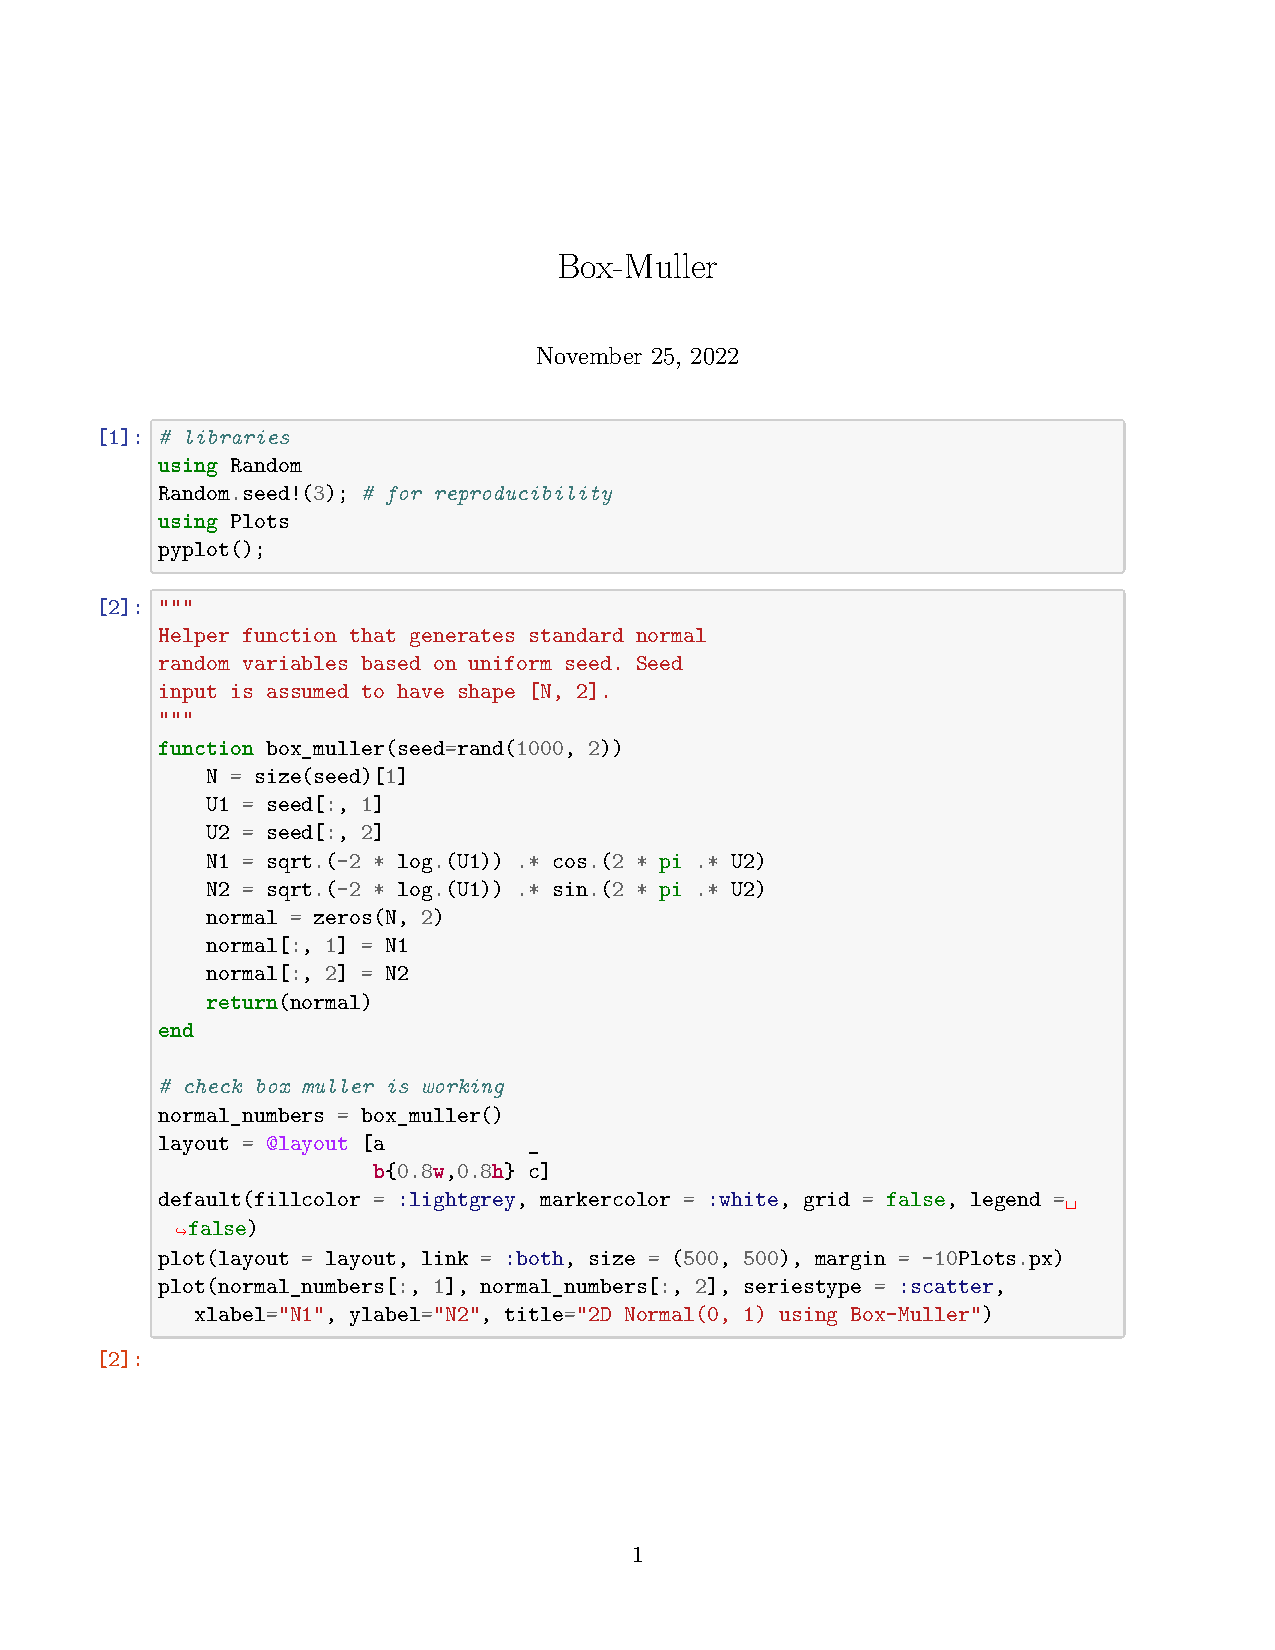
\includepdf[pages=-]{proj1/Box-Muller.pdf}



\subsubsection{Extension} Is it possible to generate a pair of real random numbers $X_1,X_2$ (not necessarily Gaussian) with $\mu = 0$ and covariance structure: $\expect{X_1^2} = 1, \expect{X_2^2} = 1/3, \expect{X_1X_2} = 1$?

\emph{Solution}: It is not possible to generate such a pair, to see this, it is enough to compute the correlation coefficient that arises from this desired statistical profile:
$$
    \rho = \frac{\mathbb{E}[X_1X_2]}{\sqrt{\text{Var}[X_1]}\cdot\sqrt{\text{Var}[X_2]}} = \frac{1}{1\cdot \sqrt{\frac13}} = \sqrt{3} > 1
$$ where in the case $\mathbb{E}[X_1] = \mathbb{E}[X_2] = 0$, $\text{Var}[X_1] = \mathbb{E}[X_1^2], \text{Var}[X_2] = \mathbb{E}[X_2^2]$.

\section{Project 2}
\subsection{SDE solution} Let $X_t = \int_0^tf(s,w)dW_s$, show that $e^{X_t}$ is a solution of the SDE:
$$
    dY_t = \frac12f^2(t,w)Y_tdt + f(t,w)Y_tdW_t
$$ and $\exp(X_t - \frac12\int_0^tf^2(s,w)ds)$ is a solution of the SDE:
$$
    dY_t = f(t,w)Y_tdW_t
$$

\emph{Solution}: We recall the most general Ito's formula (scalar valued process); we will be using this formula throughout. Suppose $X_t$ satisfies the integral form:
$$
    X_t = X_0 + \int_0^tA_sds + \int_0^tC_sdB_s
$$ and suppose $f(t,x)$ is $C^1$ in $t$, and $C^2$ in $x$, Ito's formula gives:
$$
    df(t,X_t) = \bigg[
        \partial_tf(t,X_t) + A_t\partial_xf(t,X_t) + \frac12C_t^2\partial_{xx}f(t,X_t)
    \bigg]dt + C_t\partial_xf(t,X_t)dB_t
$$ where $B_t$ is standard Brownian motion (sBM); our text uses $W_t$.

The first problem is a verification of Ito's formula. Here $X_t = \int_0^tf(s,\omega)dW_s$. Then:
$$
    dX_t = f(t,\omega)dW_t
$$

Let $Z_t = \exp(X_t)$, the exponential function is smooth in $x$, then applying Ito's formula we obtain:
$$
    dZ_t = \frac12f^2(t,\omega)\exp(X_t)dt + f(t,\omega)\exp(X_t)dW_t
$$
$$
    = \frac12f^2(t,\omega)Z_tdt + f(t,\omega)Z_tdW_t
$$ thus the first part is verified.

Similarly, let now:
$$
    Z_t = e^{X_t - \frac12\int_0^tf^2(s,\omega)ds}
$$

The function $g(t,x) = e^{x-\frac12\int_0^tf^2(s,\omega)ds}$ is $C^1$ in $t$ and smooth in $x$, and:
$$
    \frac{\partial}{\partial t}g(t,x) =  \frac{\partial}{\partial t}\bigg[
        e^{x}\cdot e^{-\frac12\int_0^tf^2ds}
    \bigg]
$$
$$
    = -\frac12f^2(t,\omega)\exp(x-\frac12\int_0^tf^2ds) = -\frac12f^2(t,\omega)g(t,x)
$$
$$
    \partial_xg(t,x) = \partial_{xx}g(t,x) = g(t,x)
$$

Then:
$$
    dZ_t = dg(t,X_t) = \bigg[
        \partial_tg(t,X_t) + \frac12f^2(t,\omega)\partial_{xx}g(t,X_t)
    \bigg]dt + f(t,\omega)\partial_xg(t,X_t)dW_t
$$
$$
    = \bigg[
        \underbrace{-\frac12f^2(t,\omega)Z_t + \frac12f^2(t,\omega)Z_t
    \bigg]dt}_{=0} + f(t,\omega)Z_tdW_t
$$

\subsection{Langevin equation} Derive the second moment equation for general linear Ito SDE, and find first and second moments of the Langevin equation.

\emph{Solution}: The general linear Ito SDE has form:
$$
    dX_t = (a_1(t)X_t+a_2(t))dt + (b_1(t)X_t+b_2(t))dW_t
$$ 

And integral form:
$$
    X_t = X_0 + \int_0^t(a_1(s)X_s + a_2(s))ds + \int_0^t(b_1(s)X_s + b_2(s))dW_s
$$

Define $m(t) = E[X_t]$, then taking expectation on both sides of the integral form (assuming bounded total variation), we have:
$$
    m(t) = E[X_0] + \int_0^ta_1(s)E[X_s]ds + \int_0^ta_2(s)ds + 0
$$ the zero comes from the fact that Ito integral is a martingale (see proof in Chapter 3 of textbook).

Differentiating both sides with respect to $t$ yields:
$$
    m'(t)  = a_1(t)m(t) + a_2(t)
$$

Now define $Y_t = f(X_t) = X_t^2$; $f$ is $C^2$ in $x$, therefore we use Ito's formula again:
$$
    dY_t = \bigg[
     2(a_1(t)X_t + a_2(t))\cdot X_t + (b_1(t)X_t+b_2(t))^2
    \bigg]dt + 2(b_1(t)X_t+b_2(t))X_tdW_t
$$
$$
    = \bigg[
        (2a_1 + b_1^2)X_t^2 + (2a_2 + 2b_1b_2)X_t + b_2^2
    \bigg]dt + (2b_1X_t^2 + 2b_2X_t)dW_t
$$

The integral form:
$$
    Y_t = Y_0 + \int_0^t[(2a_1+b_1^2)X_s^2 + (2a_2 + 2b_1b_2)X_s +b_2^2]ds + \int_0^t[2b_1X_s^2 + 2b_2X_s]dW_s
$$

Let $D(t)$ denote $E[Y_t] = E[X_t^2]$, then:
$$
    D(t) = E[X_0^2] + \int_0^t[(2a_1+b_1^2)D(s) + (2a_2+2b_1b_2)m(s) + b_2^2]ds + 0
$$
$$
    D(t) = E[X_0^2] + \int_0^t(2a_1(s) + b_1^2(s))D(s)ds + \int_0^1(2a_2(s) + 2b_1(s)b_2(s))m(s)ds + \int_0^tb_2^2(s)ds
$$

Take derivative with respect to $t$ on both sides, the constant terms vanish, and:
$$
    D'(t) = [2a_1(t) + b_1^2(t)]D(t) + [2a_2(t) + 2b_1(t)b_2(t)]m(t) + b_2^2(t)
$$ the solution can also be found on textbook page 113, equation (2.11).

The Langevin equation reads:
$$
    dX_t = -aX_tdt + bdW_t
$$

Let $m(t) = E[X_t]$, then taking expectation on both sides:
$$
    E[X_t] = E[X_0] - a\int_0^tE[X_s]ds\Leftrightarrow m(t) = E[X_0] - a\int_0^tm(s)ds 
$$ then:
$$
    m'(t) = -am(t)
$$
Integral form:
$$
    X_t = X_0-a\int_0^tX_sds + b\int_0^tdW_s
$$ which has the analytic solution:
$$
    m(t) = m(0)\cdot e^{-at} = E[X_0]\cdot \exp(-at)
$$

Define $Y_t = X_t^2$, then:
$$
    dY_t = [-2aX_t^2 + b^2]dt + 2bX_tdW_t = [-2aY_t + b^2]dt + 2bX_tdW_t
$$
$$
    Y_t = Y_0 + \int_0^t(-2aY_s + b^2)ds + 2b\int_0^tX_sdW_s
$$
$$
    E[Y_t] = E[Y_0] -2a\int_0^tE[Y_s]ds + b^2\int_0^tds + 0
$$
$$
    E[Y_t] = E[Y_0] - 2a\int_0^tE[Y_s]ds + b^2t
$$
$$
    D'(t) = \frac{d}{dt}E[Y_t] = -2aD(t) + b^2
$$
This ODE has analytic solution:
$$
    D(t) = \frac{b^2}{2a} + (E[X_0^2] - \frac{b^2}{2a})e^{-2at}
$$


\subsection{OU process generation} Generate the Ornstein-Uhlenbeck process numerically by discretizing the integral representation:
$$
    X_t = e^{-2t}X_0 + 2\int_0^te^{-2(t-s)}dW_s
$$ with left hand rule (which yields Ito), for a small grid size $ds$, for $t\in [0,1]$. Here $X_0$ is a $\mathcal{N}(0,1)$ random variable independent of the Brownian path $W_t,t>0$. 

Compute the covariance $\expect{X_tX_s}$ numerically, and compare with the exact covariance $e^{-2\abs{t-s}}$, to help guide choosing a good choice of $ds$. 

Plot a sample path of the solution on $[0,1]$.

\emph{Solution}: The derivation and code are as follows.

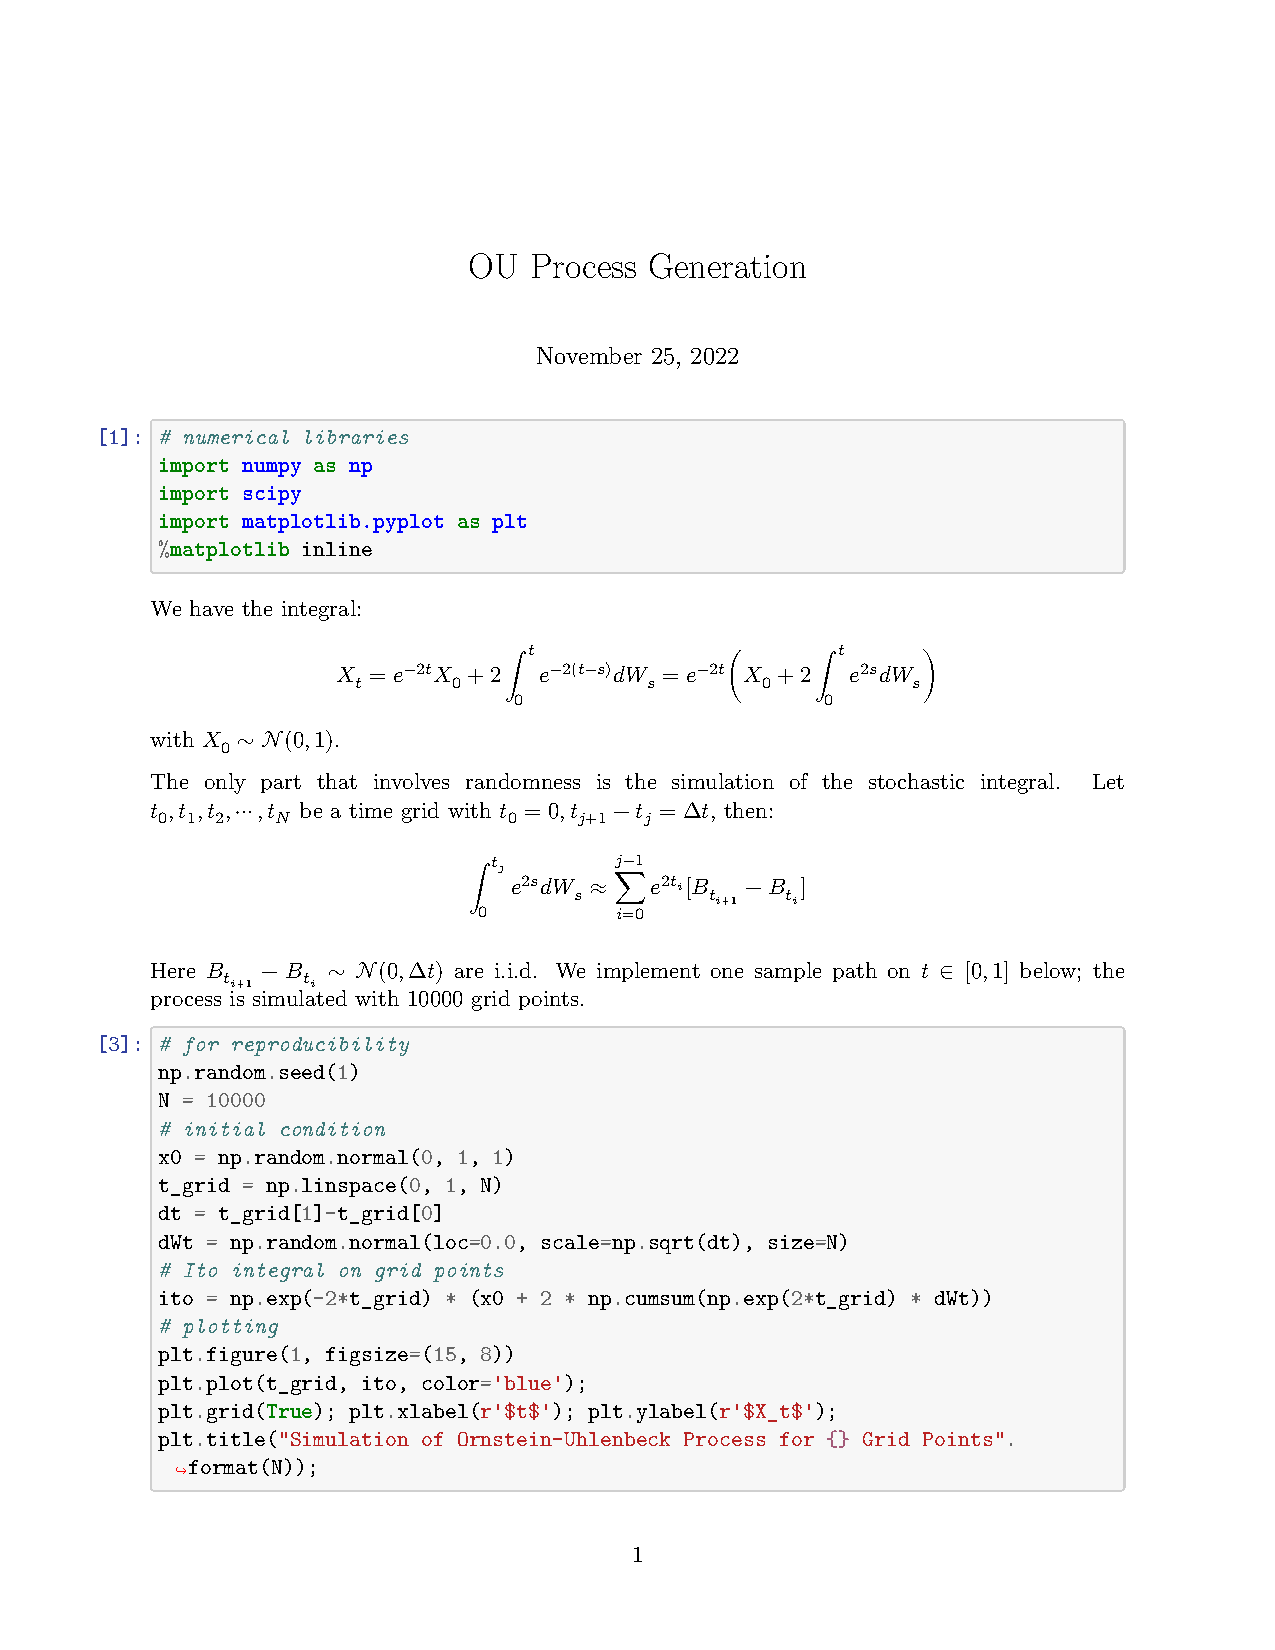
\includepdf[pages=-]{proj2/OU Process Generation.pdf}

\section{Project 3}
\subsection{Convergence of Linear SDE} Consider the SDE:
$$
    dX_t=aX_tdt + bX_tdW_t
$$ with $a, b$ constant. Discretize the SDE with Euler scheme and find the order of convergence for its third and fourth order moments.

\emph{Solution}: More details can be found in the textbook section 9.7. We say a discrete time approximation $Y^{\delta}$ converges to $X$ weakly at time $T$ as $\delta\downarrow 0$ with respect to a class $\mathcal{C}$ of test functions if:
$$
    \lim_{\delta\rightarrow 0}|E(g(X_T)) - E(g(Y^{\delta}(T)))| = 0
$$ for all $g\in\mathcal{C}$. Furthermore, $Y^{\delta}$ is said to converge weakly with order $\beta>0$ if for each $g\in\mathcal{C}_P^{2(\beta+1)}(\mathbb{R}^d,\mathbb{R})$ (the class of 2($\beta+1$) times differentiable functions) if there is a constant $C>0,\delta_0<\infty$ such that:
$$
|E[g(X_T)] - E[g(Y^{\delta})]| \le C\delta^{\beta}
$$ for all $\delta\in (0,\delta_0)$.

From Theorem 9.7.4 we can verify that our constant coefficient SDE satisfies the assumptions with Euler scheme. Theorem 14.1.5 shows that Euler is at least order $\beta = 1$ weakly convergent. Thus we have:
$$
    |E[g(X_T)] - E[g(Y^{\delta})]| \le C\delta
$$ for all $g\in \mathcal{C}_P^{4}$. Let $g_1(x) = x^3, g_2(x) = x^4$, it is clear that $g_1,g_2\in\mathcal{C}_P^{4}$. On the other hand, this shows:
$$
    |E[X_T^3] - E[(Y^{\delta})^3]| \le C\delta, |E[X_T^4] - E[(Y^{\delta})^4]| \le C\delta
$$ 

Respectively, this implies that the third and fourth moments of $Y^{\delta}$ are order-1 convergent. Note that it is incorrect to say ``weak convergence'' here because third and fourth moments are deterministic.


\subsection{Propagating Front IBVP} Consider the initial-boundary value problem:
$$
    u_t = 0.0025u_{xx} + e^{\xi(x,w)}u(1-u), x\in[0,15]
$$
$$
    u(t,0) = 1, u(t,15) = 0, u(0,x) = \chi_{[0,1]}(x)
$$ where $\xi(x,w)$ is the OU process with $\mathcal{N}(0,1)$ as initial condition, and covariance $\expect{\xi(x)\xi(0)}=e^{-2x}$. Use backward time centered in space scheme with proper stepsizes $h, k$ $(h\le 0.01)$ to discretize the PDE. 





\subsubsection{Sample solutions} Plot sample solutions of $u$ for $t=0,4,8,12,16,20$. 

\subsubsection{Sample generation} Generate $N\ge 1000$ samples. For each ensemble solution $u(\cdot , \cdot ; \omega)$, define another random process:
$X_t(\omega)$ such that $u(X_t(\omega),t;\omega) = 1/2$. Plot a histogram of $\eta_1(\omega) = X_{20}(\omega)/20$.

\subsubsection{Summary statistic} Compute $c = \expect{\eta_1}$ and:
$$
    c' = 2\sqrt{0.025 \cdot \expect{e^{\xi}}}
$$ $c'$ is a naive estimate of the random front velocity. Compare $c$ and $c'$.

\emph{Solution}: The derivation of finite differencing and Python code are as follows.
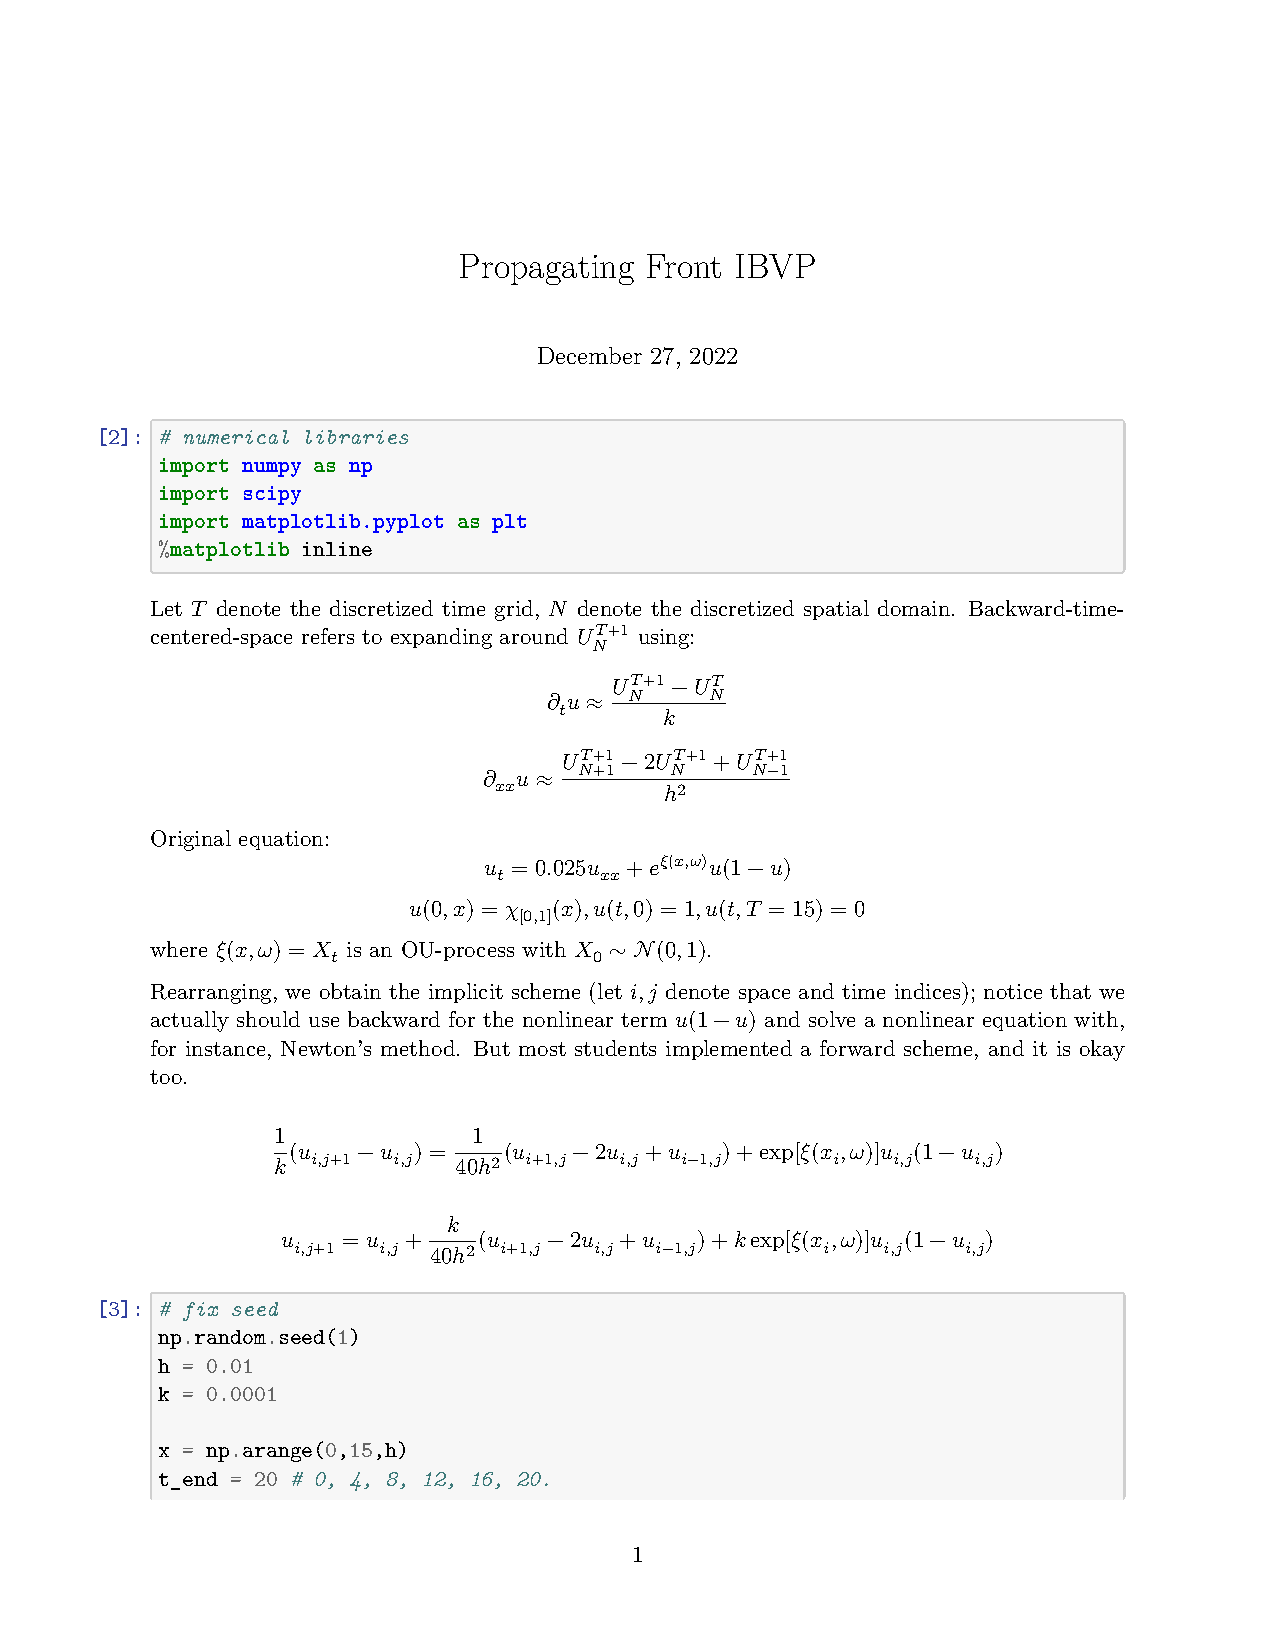
\includepdf[pages=-]{./proj3/Propagating Front IBVP.pdf}


\subsection{SDE solution} Consider the SDE:
$$
    dX_t = aX_tdt + bX_tdW_t
$$ which has exact solution:
$$
    X_t = X_0\exp((a-\frac{b^2}{2})t+bW_t)
$$ let $X_0=1$, $a=1.5,b=1$, solve the above SDE using Euler and Milstein schemes for $t$ up to $1$, using time discretizations $\delta = 2^{-3}, 2^{-4}, 2^{-5}, 2^{-6}$.

\subsubsection{Visualization} Plot and compare sample solutions together with the exactly  solution.

\subsubsection{Sample generation} Generate 20000 samples for each value of $\delta$, and compute the absolute error $\eps = \expect{\abs{X(1)-Y_{\delta}(1)}}$, where $Y_{\delta}(1)$ is the final solution at $t=1$ numerically computed with discretization level $\delta$. Plot $\epsilon(\delta)$ against different choices of $\delta$, and discuss the order of accuracy of Euler method and Milstein method.

\emph{Solution}: (Presented on the next page)
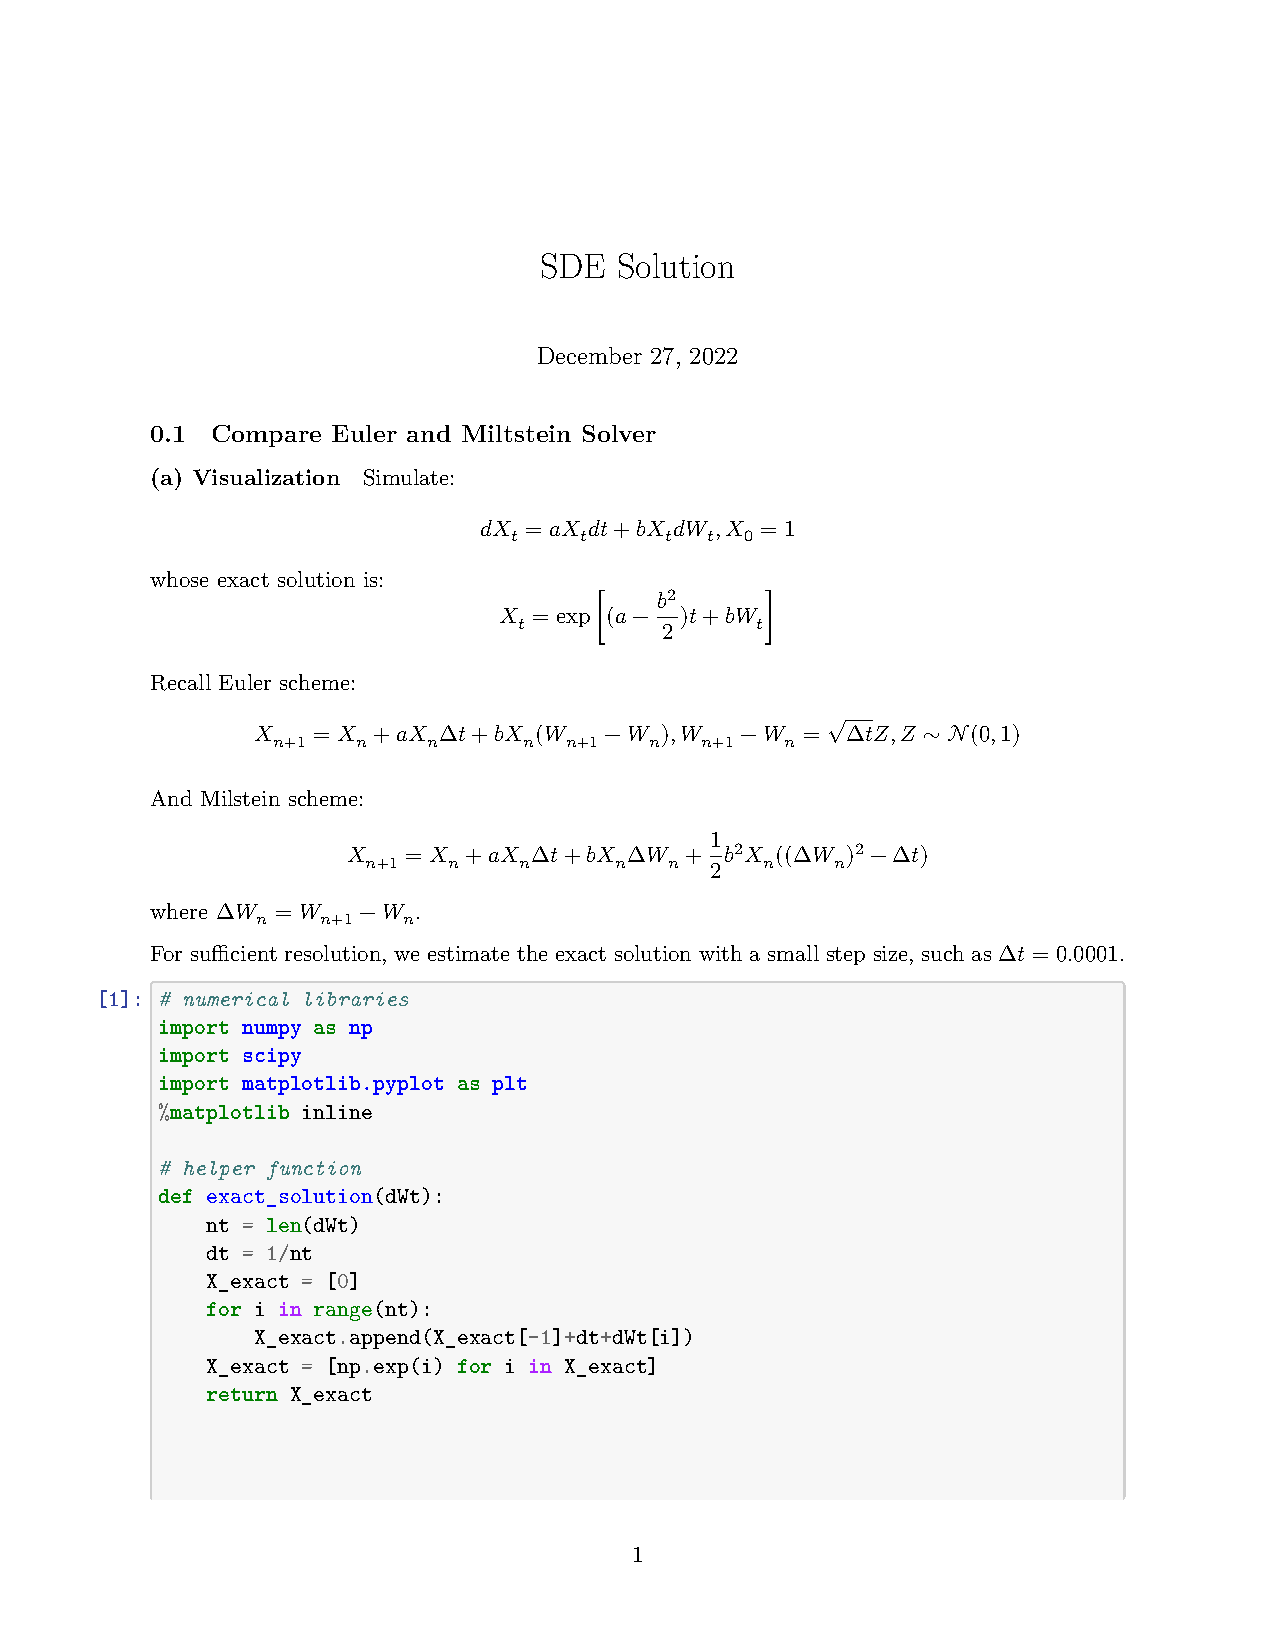
\includepdf[pages=-]{./proj3/SDE Solution.pdf}



\section{Project 4}
\subsection{Multiple dimensional Wiener process} Given:
$$
    dX_t = adt + \sum_{j=1}^mb^jdW_t^j
$$ determine:
$
    \underline{f}_{(j_1,j_2,j_3,j_4)}
$ and $ f_{(j_1,j_2,j_3,j_4)}$ for $j_1,j_2,j_3,j_4\in\{1,\ldots,m\}$.

\emph{Solution}: 

We have:

$$
    dX = adt + \sum_{j=1}^mb^jdW^j
$$ Please see Lecture 8 and Lecture 10 for a detailed discussion of the simplified notations (Ito-Taylor and Stratonovich-Taylor forms). The solution to this question is quite mechanical and it is enough to carry out the recursive definition. Note that $b^j$ is indexing the coefficient for each process, not power.

$$
    f_{\alpha} = 
    \begin{cases}
        f: l=0\\
        L^{j_1}f_{-\alpha}, l\ge 1
    \end{cases}
$$ where:
$$
    L^j = \sum_{k=1}^db^{k,j}\frac{\partial}{\partial x^k} = b^j\frac{\partial}{\partial x}
$$ here $d=1$, thus the last equality.

$$
    L^0 = \frac{\partial}{\partial t} + a\frac{\partial}{\partial x} + \frac12\sum_{j=1}^m (b^j)^2\frac{\partial^2}{\partial x^2}
$$

Thus:
$$
    f_{(j_1,j_2,j_3,j_4)} = L^{j_1}f_{(j_2,j_3,j_4)} = \cdots = L^{j_1}L^{j_2}L^{j_3}L^{j_4}f
$$ and notice $j_1,j_2,j_3,j_4\ge 1, f(t,x)=x, \frac{\partial f}{\partial x} = 1$:
$$
    L^{j_4}f = b^{j_4}
$$
$$
    L^{j_3}(L^{j_4}f) = L^{j_3}(b^{j_4}) = b^{j_3}\frac{\partial}{\partial x}b^{j_4} = b^{j_3}b^{j_4'}
$$
$$
    L^{j_2}(L^{j_3}L^{j_4}f) = L^{j_2}(b^{j_3}b^{j_4'}) = b^{j_2}\frac{\partial}{\partial x}b^{j_3}b^{j_4'} = b^{j_2}(b^{j_3'}b^{j_4'} + b^{j_3}b^{j_4''}) = b^{j_2}b^{j_3'}b^{j_4'} + b^{j_2}b^{j_3}b^{j_4''}
$$
$$
    f_{\alpha} = L^{j_1}b^{j_2}b^{j_3'}b^{j_4'} + L^{j_1}b^{j_2}b^{j_3}b^{j_4''} = b^{j_1}\frac{\partial}{\partial x}(b^{j_2}b^{j_3'}b^{j_4'}+b^{j_2}b^{j_3}b^{j_4''})
$$
$$
    \frac{\partial}{\partial x}b^{j_2}b^{j_3'}b^{j_4'} = b^{j_2'}b^{j_3'}b^{j_4'} + b^{j_2}b^{j_3''}b^{j_4'} +b^{j_2}b^{j_3'}b^{j_4''} 
$$
$$
    \frac{\partial}{\partial x}b^{j_2}b^{j_3}b^{j_4''} = b^{j_2'}b^{j_3}b^{j_4''} + b^{j_2}b^{j_3'}b^{j_4''} + b^{j_2}b^{j_3}b^{j_4'''}
$$

Finally:
$$
    f_{\alpha} = b^{j_1}(b^{j_2'}b^{j_3'}b^{j_4'} + b^{j_2}b^{j_3''}b^{j_4'} + 2b^{j_2}b^{j_3'}b^{j_4''} + b^{j_2}b^{j_3}b^{j_4''} + b^{j_2}b^{j_3}b^{j_4'''})
$$ The Stratonovich-Ito case is omitted.

\subsection{Approximation of stochastic integral} Consider:
$$
    W_1^1I_{(1,2)}[1]_{0,1}
$$
\subsubsection{Random coefficients} Find a representation of $I_{(1,2)}$ in terms of some random coefficients.

\emph{Solution}: 
$$
    l((1,2)) = 2
$$ thus:
$$
    I_{(1,2)} = J_{(1,2)} - \frac12I_{\{j_1=j_2\neq 0\}}J_{(0)} = J_{(1,2)}
$$ because $j_1\neq j_2$.
$$
    J_{(1,2)} = \frac12W_{\Delta}^{1}W_{\Delta}^2-\frac12(a_{2,0}W^1_{\Delta} - a_{1,0}W_{\Delta}^2) + \Delta(\frac{\pi}{\Delta}\sum_{r=1}^{\infty} r(a_{1,r}b_{2,r} - b_{1,r}a_{2,r}))
$$ Here the coefficients $a_{i,j}, b_{i,j}$ are normally distributed and pairwise independent.

\subsubsection{Monte Carlo} Compute $\expect{W_1^1I_{(1,2)}[1]_{0,1}}$ with Monte Carlo based on a truncation of part 1.

\emph{Solution}: (See next page)
\subsubsection{Direct simulations} Compute $\expect{W_1^1I_{(1,2)}[1]_{0,1}}$ again directly using Wiener process samples and integrating along the paths.

\emph{Solution}: (See next page)

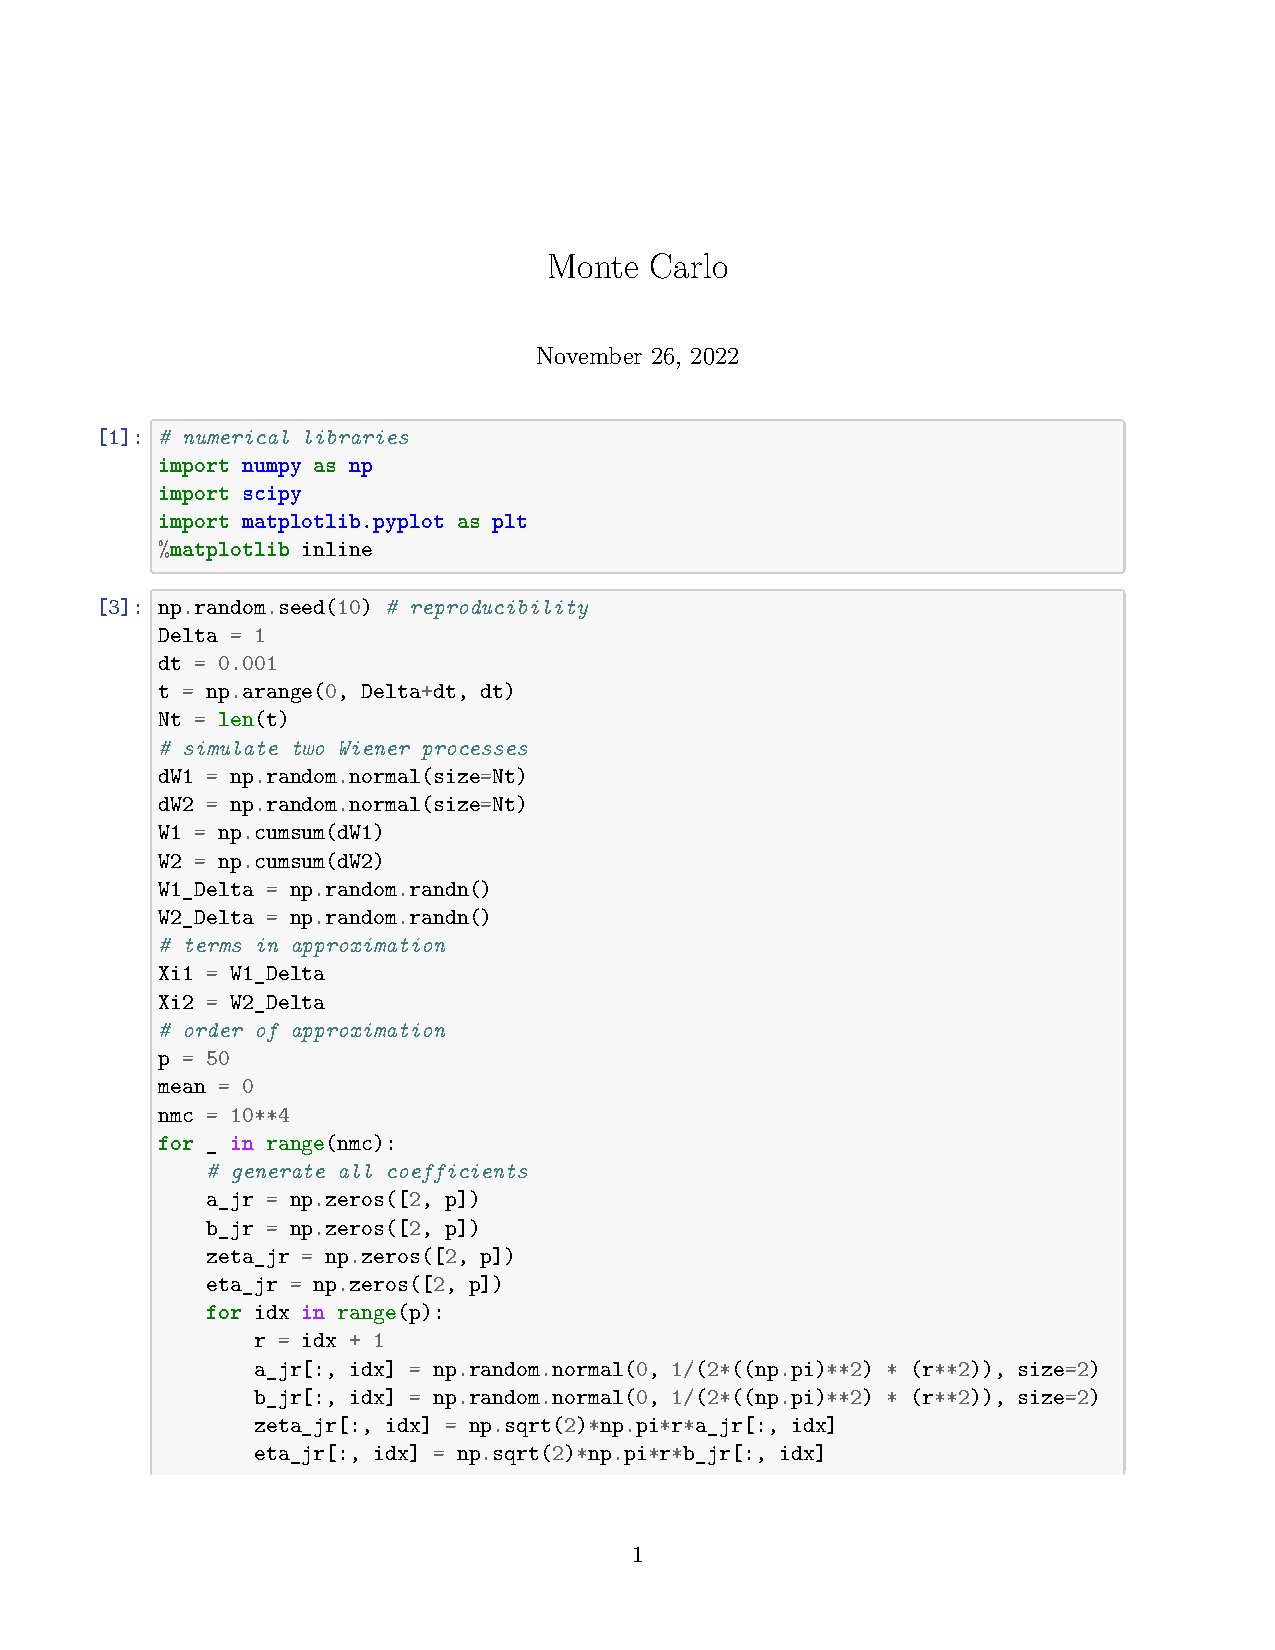
\includepdf[pages=-]{./proj4/Monte Carlo.pdf}
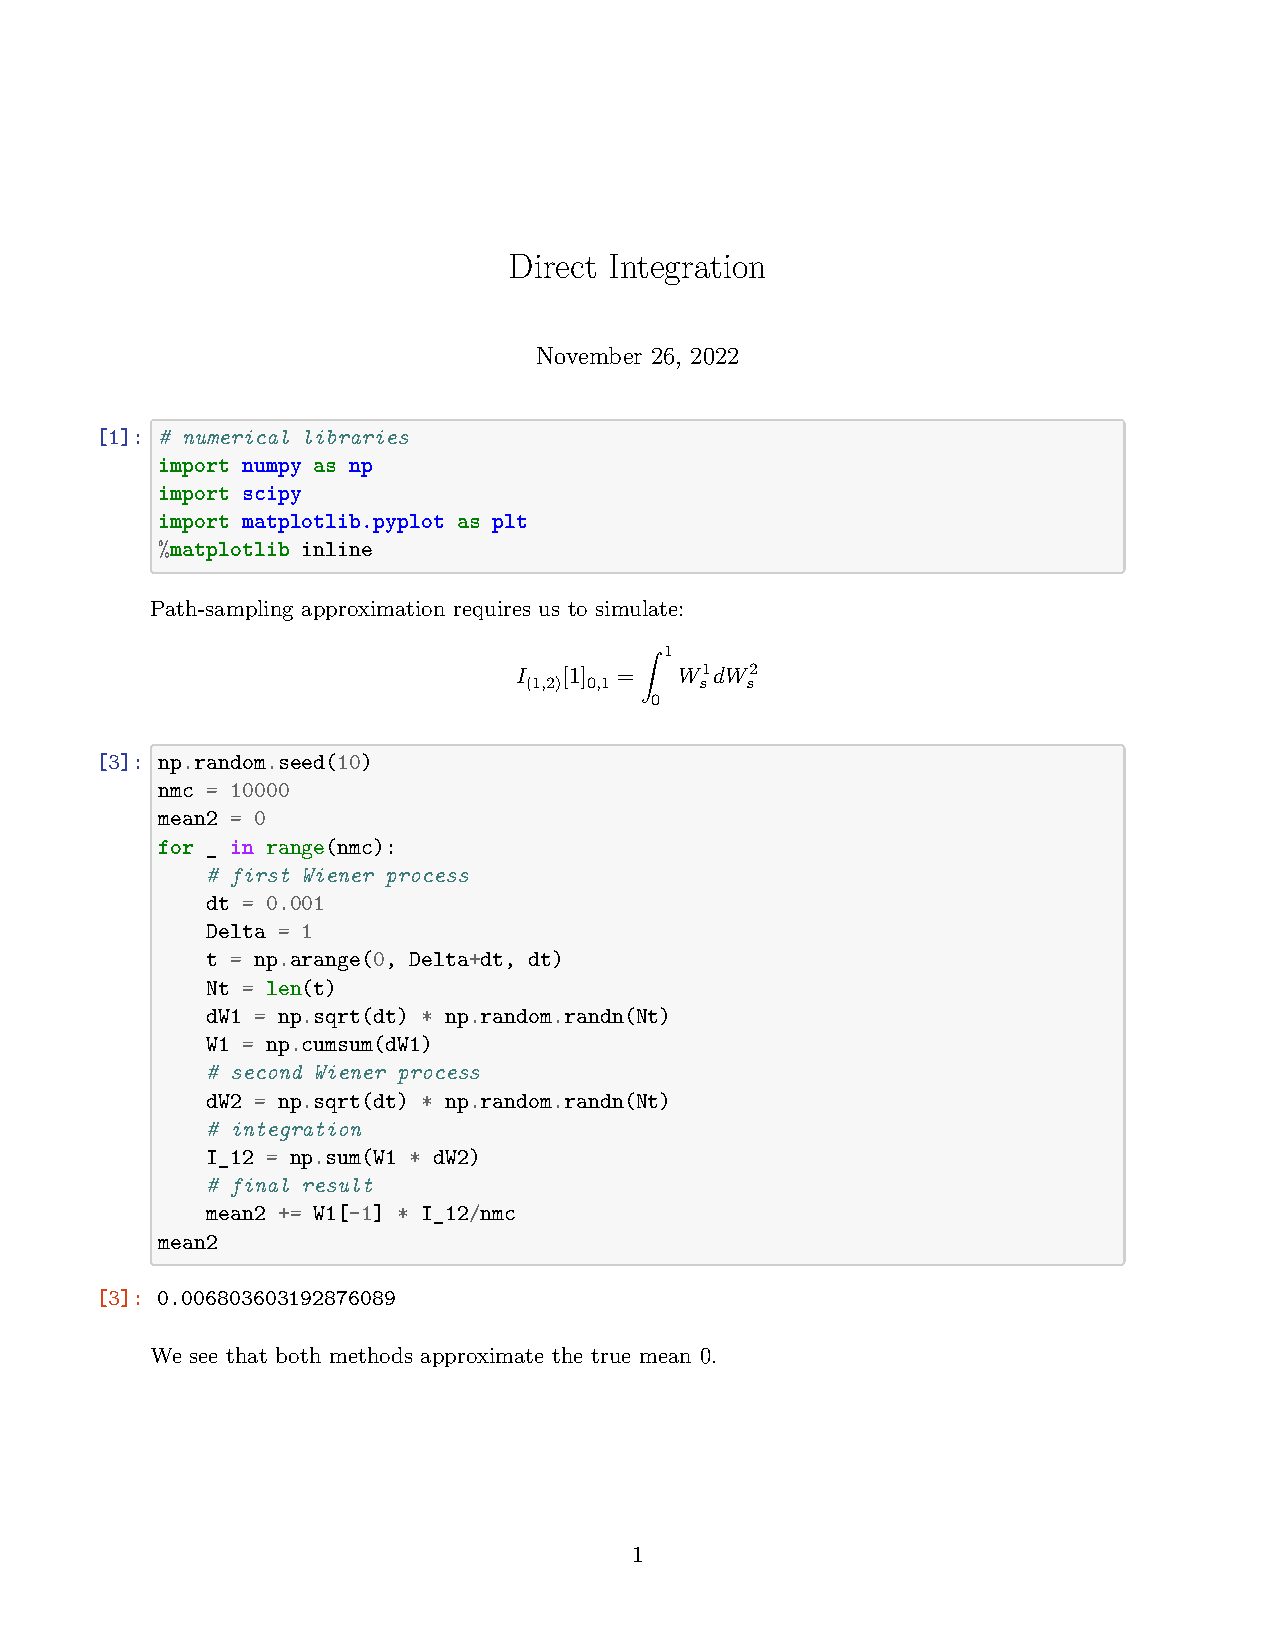
\includepdf[pages=-]{./proj4/Direct Integration.pdf}

\section{Project 5}
\subsection{$L^p$ strong convergence} Finish the proof of $L^p$ strong convergence.

\emph{Solution sketch}: Follow the proof for the $L^2$ case in Platen 10.7. For the $L^p$ generalization, one may cite \href{https://en.wikipedia.org/wiki/Doob\%27s_martingale_inequality}{Doob's maximal inequality for submartingales in $L^p$} on $X_t - Y^{\delta}(t)$, and derive an analogous inequality as (7.7), then apply the tower property on both sides by taking expectations.

\subsection{SDE problem} For $t\ge t_0=0$, consider:
$$
    dX_t = (\frac{2}{1+t}X_t + (1+t)^2)dt + (1+t)^2dW_t
$$ with $X_0=1$.

\subsubsection{Exact solution} Verify that it has an exact solution:
$$
    X_t = (1+t)^2(1+W_t+t)
$$

\emph{Solution}: We use Ito formula to take the differential of $X_t$:
$$
    dX_t = \big[3(1+t)^2+2(1+t)W_t\big]dt + (1+t)^2dW_t
$$ and noting that:
$$
    \frac{2}{1+t}X_t + (1+t)^2 = 3(1+t)^2 + 2(1+t)W_t
$$ we conclude that the solution indeed matches, with $X_0 = 1\cdot (1+0+0) = 1$. 
\subsubsection{Approximation of final solution} Approximating $X_T$ with the Chang scheme, for $T=0.5$, in which $J_{(1,1,0)}$ is approximated by $J_{(1,1,0)}^p$ for $p=15$. Make this approximation for equal step sizes $\delta = 2^{-1}, 2^{-2}, 2^{-3}, 2^{-4}, 2^{-5}$ and record the absolute error. 

\emph{Solution}: Recall the nonautonomous Chang scheme (Chapter 11, Platen):
\begin{equation}\label{eqn:chang-scheme}
    Y_{n+1} = Y_n + \frac12\bigg[
        a(t_n + \frac12\Delta t,\bar{Y}_+) + a(t_n + \frac12\Delta t,\bar{Y}_-)
    \bigg]\Delta t
\end{equation}
$$
    + b(t_n)\Delta W + \frac{1}{\Delta t}(b(t_{n+1}) - b(t_n))\cdot (\Delta W\Delta t - \Delta Z)
$$ where:
$$
    \bar{Y}_{\pm} = Y_n + \frac12\underline{a}(t_n,Y_n)\Delta t + \frac{1}{\Delta t}\cdot b(t_n)\bigg[
        \Delta Z \pm \sqrt{2J_{(1,1,0)}\Delta t - (\Delta Z)^2}
    \bigg]
$$ and $\underline{a}$ is the Stratonovich corrected drift:
$$
    \underline{a} = a - \frac12bb'
$$

In this question, we approximate $J_{(1,1,0)}$ as described in Exercise 10.5.1 of Platen, with $p=15$:
$$
    J_{(1,1,0)} \approx J_{(1,1,0)}^p = \frac{1}{3!}(\Delta t)^2\zeta_1^2+\frac14(\Delta t)a_{1,0}^2 - \frac{1}{2\pi}(\Delta t)^{3/2}\zeta_1b_1 
$$
$$+ \frac14(\Delta t)^{3/2} a_{1,0}\zeta_1 - (\Delta t)^2C_{1,1}^p
$$ And:
$$
    C_{1,1}^p = -\frac{1}{2\pi^2}\sum_{r,l=1,r\neq l}^p\frac{r}{r^2-l^2}\bigg(
        \frac{1}{l}\xi_{1,r}\xi_{1,l} - \frac{l}{r}\eta_{1,r}\eta_{1,l}
    \bigg)
$$ with the following definitions:
$$
    \begin{cases}
        a_{1,0} = -\frac{1}{\pi}\sqrt{2\Delta t}\sum_{r=1}^p\frac{1}{r}\xi_{1,r} - 2\sqrt{(\Delta t)\rho_p}\mu_{1,p}\\
        \rho_p = \frac{1}{12}-\frac{1}{2\pi^2}\sum_{r=1}^p\frac{1}{r^2}\\
        b_1 = \sqrt{\frac{\Delta t}{2}}\sum_{r=1}^p\frac{1}{r^2}\eta_{1,r} + \sqrt{(\Delta t)\alpha_p}\phi_{1,p}\\
        \alpha_p = \frac{\pi^2}{180}-\frac{1}{2\pi^2}\sum_{r=1}^p\frac{1}{r^4}
    \end{cases}
$$ here $\zeta_1, \xi_{1,r}, \eta_{1,r}, \mu_{1,p}, \phi_{1,p}$ for $r=1,\ldots, p$ are independent standard Gaussian random variables.

The code that implements the Chang scheme is on the next page, along with the exact sample paths.

\subsubsection{Visualization} Plot the absolute error against $\log_2\delta$ and explain order of convergence.

\emph{Solution}: The plotting is omitted. One may investigate its strong order of convergence by computing an average absolute final error.

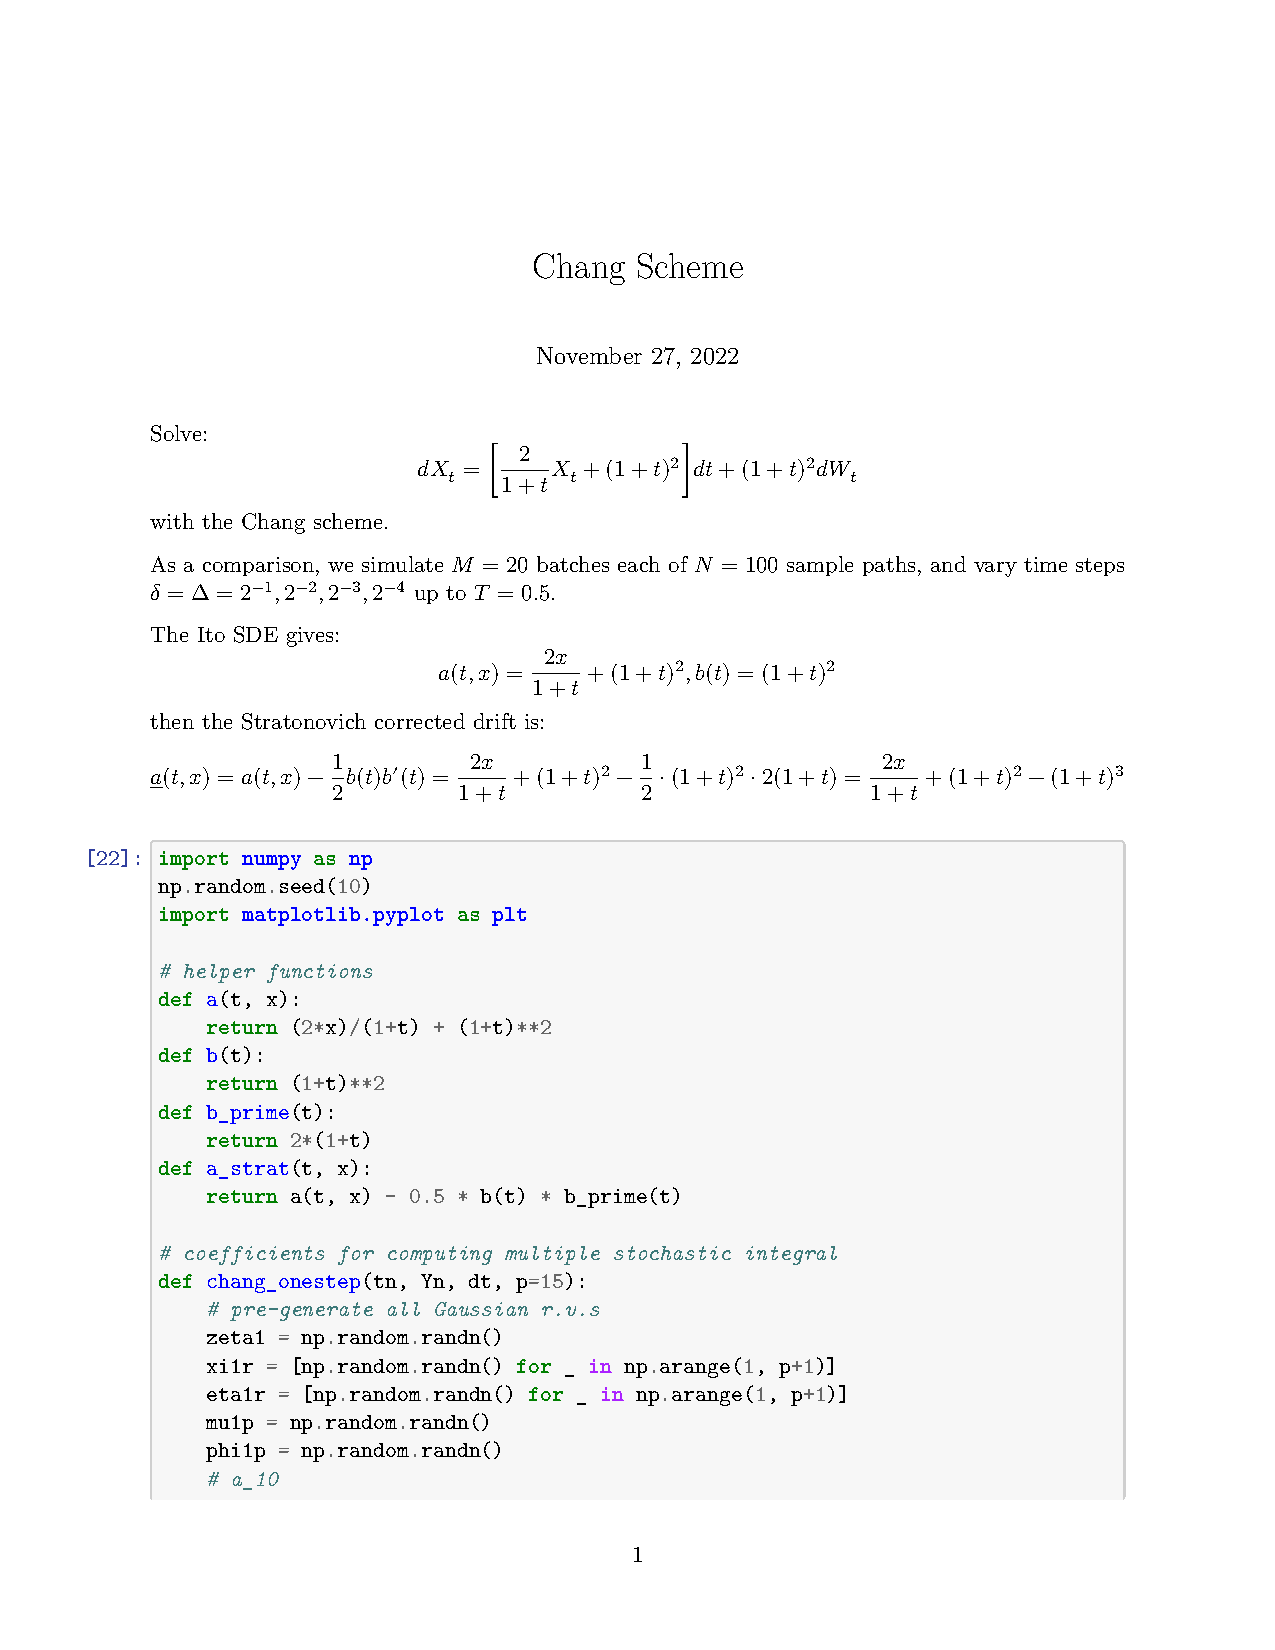
\includepdf[pages=-]{proj4/Chang Scheme.pdf}

\section{Final (Partial)}
\subsection{Multiple Brownian Motions}
Consider $1$D SDE driven by two independent Wiener processes:
\begin{equation}
    dX_t = X_tdt + X_tdW_t^1 + X_tdW_t^2, X_0 = 1
\end{equation}
\subsection{Strong solution} We may consider thie as a generalization of Lecture 4, part 4 for general linear SDEs. We first change the two stochastic differentials into Stratonovich form:
\begin{equation}
    dX_t = (X_t - 2\cdot\frac12X_t)dt + X_t\circ dW_t^1 + X_t\circ dW_t^2
\end{equation}
$$
     = X_t\circ dW_t^1 + X_t\circ dW_t^2
$$

Then following (4.13)-(4.16), 
$$
    \Phi_{0,t} = \exp\bigg(
        \int_0^tdW_s^1 + \int_0^tdW_s^2
    \bigg) = \exp\bigg(
        W_t^1 + W_t^2
    \bigg)
$$ Since $X_0=1$, we have:
\begin{equation}
    X_t = \exp\bigg(
        W_t^1 + W_t^2
    \bigg)
\end{equation}

\subsection{Integral form and Expectation} The integral form reads:
$$
    X_t = 1 + \int_0^tX_sds + \int_0^tX_sdW_s^1 + \int_0^tX_sdW_s^2
$$

To compute $\expect{X_T}$, since $W_t^1,W_t^2$ are independent Wiener processes, $W_T^1, W_T^2$ are i.i.d. $\mathcal{N}(0,T)$ random variables. Then:
\begin{equation}
    \expect{X_T} = \expect{\exp(W_T^1+W_T^2)} = \expect{\exp(W_T^1)}\cdot\expect{\exp(W_T^2)}
\end{equation} Since $W_T^1$, $W_T^2$ are normal random variables, $\exp(W_T^1),\exp(W_T^2)$ are log-normally distributed. Therefore we conclude the expectation is the following (using the formula derived from the log-normal density):
\begin{equation}
    \expect{X_T} = (e^{\frac12T})^2 = e^T
\end{equation}

\end{document}
